\documentclass{article}
\usepackage{graphicx} 
\usepackage[T2A]{fontenc}    
\usepackage[utf8]{inputenc}  
\usepackage[english,russian]{babel}
\usepackage{multicol}
\usepackage{amsmath} 
\usepackage{wrapfig}
\usepackage{footnote} 

\begin{document}
\begin{multicols}{2}

Проходит через точку $O$ и наоборот. То, что мы говорили, можно выразить и при помощи формул.

Из рисунка 6а видно, что
\[
\begin{cases}
x = OB = a \cos \varphi = a \cos \omega t, \\
y = OC = a \sin \varphi = a \sin \omega t = \\
\quad = a \cos \left( \omega t - \frac{\pi}{2} \right) = a \cos \omega \left( t - \frac{T}{4} \right).
\end{cases}
\tag{1}
\]
Формулы (1) справедливы при любом угле, а не только при остром. (Это следует из определений косинуса и синуса).

Если движение точки $A$ происходит по часовой стрелке (рис. 6б), то, проследив за движениями точек $C$ и $B$ на четверть периода, можно сказать, что колебание точки $C$ на три четверти периода отстает от колебания точки $B$. Так как в этом случае угол $\omega t$ считается отрицательным, то
\[
\begin{cases}
x = a \cos(-\omega t) = a \cos \omega t, \\
y = a \sin(-\omega t) = -a \sin \omega t = \\
\quad = a \cos\left(\omega t + \frac{\pi}{2}\right) = a \cos\left(\omega t - \frac{3\pi}{2}\right) = \\
\quad = a \cos\left(\omega \left(t - \frac{3T}{4}\right)\right).
\end{cases}
\tag{2}
\]
Из формул (1) и (2) видно, что координаты $x$ и $y$ периодически меняются с течением времени $t$. Это означает, что точки $B$ и $C$ совершают колебательные движения.
\begin{center}
    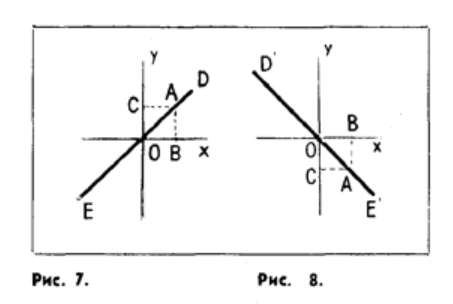
\includegraphics[width=0.8\columnwidth]{image.png} 
\end{center}
Пусть теперь точка $A$ вместо движения совершает гармонические колебания вдоль прямой $EOD$ (рис. 7) с амплитудой $b$, $OD = OE$. В этом случае обе проекции $B$ и $C$ колеблются и одновременно достигают наибольших отклонений в положительных и отрицательных направлениях осей $x$ и $y$, одновременно проходя через точку $O$. Точки $B$ и $C$, как говорят, колеблются «в фазе». При этом амплитуды колебаний точек $B$ и $C$ одинаковы и равны:
\[
b \cos \frac{\pi}{4} = b \sin \frac{\pi}{4} = \frac{b}{\sqrt{2}}.
\]

Поскольку $OB = b \cos \omega t$, получаем
\[
x = y = \frac{b}{\sqrt{2}} \cos \omega t. \tag{3}
\]
Если же точка $A$ колеблется вдоль прямой $E'D'$ (рис. 8), то в момент наибольшего отклонения точки $B$ в положительном направлении оси $x$ отклонение точки $C$ имеет наибольшую величину в отрицательном направлении оси $y$. В этом случае говорят, что колебания точек $B$ и $C$ совершаются «в противофазе». Можно считать также, что колебание точки $C$ отстает от колебания точки $B$ на полпериода (или опережает на полпериода — в данном случае это все равно). Тогда
\[
\begin{cases}
x = \frac{b}{\sqrt{2}} \cos \omega t, \\
y = -\frac{b}{\sqrt{2}} \cos \omega t = \frac{b}{\sqrt{2}} \cos (\omega t - \pi) = \\
\quad = \frac{b}{\sqrt{2}} \cos \omega \left(t - \frac{T}{2}\right).
\end{cases}
\tag{4}
\]
Вернемся теперь к нашему маятнику. Если его грузик отклонить в

\begin{flushleft}
{\small \textbf{*)} Так как $\omega = \frac{2\pi}{T}$, то $\frac{\pi}{2\omega} = \frac{T}{4}$, и $y = a \cos \omega \left(t - \frac{T}{4}\right)$.}


\end{flushleft}

\end{multicols}

\end{document}
